\begin{center}{\large\bfseries Laporan 1: Analisis Perpindahan Penumpang Antarhalte}\end{center}
\addcontentsline{toc}{part}{Laporan 1: Analisis Perpindahan Penumpang Antarhalte}
\section*{Rangkuman}
Enam matriks transisi kode B untuk $N=16,32,64,128,256,512$ dipakai untuk menghitung distribusi stasioner penumpang. Sistem asal singular; satu persamaan diganti dengan syarat skala dan solusinya dinormalkan. Kami membandingkan LU dense berpivot parsial dengan eliminasi pita berpivot parsial untuk $p=2,q=1$. Pada $N=512$, solver pita memerlukan 20.09~ms dan 60~KiB, dibandingkan 164.22~ms dan 4108~KiB untuk dense. Kedua metode memberikan solusi dan residual yang sama pada ketelitian yang diamati. Kasus $N=256$ hampir terpisah menjadi dua blok dan memiliki kondisi terbesar, $\kappa_1(B)\approx1.71\times10^9$. Halte terakhir memiliki proporsi terbesar pada setiap ukuran. Untuk koridor besar, solver pita unggul dalam waktu dan memori, tetapi kondisi matriks tetap perlu dipantau.

\section{Pendahuluan dan Validasi Data}
Misalkan $X_k$ adalah halte penumpang pada interval ke-$k$ dan $T_{ij}=\Pr(X_{k+1}=j\mid X_k=i)$. Untuk setiap $N$, matriks $T$ dibaca dari CSV kode B yang sesuai dengan kelompok genap A12. Validasi memeriksa bentuk $N\times N$, elemen hingga dan nonnegatif, jumlah tiap baris satu hingga toleransi $10^{-12}$, serta keterhubungan kuat graf transisi. Dua pencarian graf, pada arah asli dan balik, memastikan rantai \emph{irreducible}; elemen diagonal positif memastikan aperiodisitas~\cite{norris}. Kondisi ini memberi distribusi stasioner tunggal dan konvergensi dari kondisi awal mana pun. Semua matriks lolos. Galat jumlah baris maksimum hanya $2.22\times10^{-16}$; setiap baris mempunyai dua sampai empat elemen tak-nol pada offset $-1,0,1,2$. Kasus $N=256$ memiliki peluang lintas blok berorde $10^{-8}$, sehingga valid namun hampir terpisah.

\begin{table}[H]\centering\small
\caption{Validasi data kode B. Semua ukuran lolos uji dimensi, nonnegativitas, jumlah baris, irreducibilitas, dan aperiodisitas.}\label{tab:validasi-ringkas}
\begin{tabular}{rrrrr}\toprule
$N$ & Galat baris maks. & $\min T_{ii}$ & $\min\{T_{ij}>0:i\ne j\}$ & Valid\\\midrule
16 & $1.11\times10^{-16}$ & 0.835 & 0.01442 & Ya\\
32 & $2.22\times10^{-16}$ & 0.835 & 0.01467 & Ya\\
64 & $2.22\times10^{-16}$ & 0.835 & 0.01483 & Ya\\
128 & $2.22\times10^{-16}$ & 0.835 & 0.01492 & Ya\\
256 & $2.22\times10^{-16}$ & 0.835 & $1.50\times10^{-8}$ & Ya\\
512 & $2.22\times10^{-16}$ & 0.835 & 0.01498 & Ya\\\bottomrule
\end{tabular}\end{table}
Tabel~\ref{tab:validasi-ringkas} memperlihatkan mengapa ukuran 256 perlu perhatian khusus: probabilitas perpindahan positif terkecil jauh lebih kecil daripada ukuran lain. Fungsi validasi juga diuji pada matriks kecil yang sengaja dibuat invalid, dan menolak nilai negatif, baris tidak stokastik, serta rantai yang tidak irreducible.

\section{Formulasi Sistem dan Struktur Pita}
Untuk vektor kolom proporsi $\pi^{(k)}$, hukum peluang total memberi $\pi^{(k+1)}=T^\mathsf{T}\pi^{(k)}$. Pada keadaan stasioner, $T^\mathsf{T}\pi=\pi$, $\mathbf1^\mathsf{T}\pi=1$, dan $\pi_i\ge0$. Dengan $A=I-T^\mathsf{T}$ diperoleh $A\pi=0$. Karena $T\mathbf1=\mathbf1$, maka $\mathbf1^\mathsf{T}A=0$: baris-baris $A$ bergantung linear dan $A$ singular. Baris pertama dapat diganti dengan syarat skala $z_1=1$:
\begin{equation}\label{eq:soal1-system}
B_{1,:}=e_1^\mathsf{T},\quad B_{i,:}=A_{i,:}\ (i\ge2),\quad b=e_1,\quad Bz=b,\quad \pi=\frac{z}{\mathbf1^\mathsf{T}z}.
\end{equation}
Untuk rantai irreducible, setiap keadaan akhirnya dapat mencapai halte 1; submatriks transisi di luar halte 1 memiliki jari-jari spektral kurang dari satu. Karena itu $B$ nonsingular~\cite{stewart}. Solusi $z$ belum berjumlah satu, sehingga normalisasi terakhir dalam~\eqref{eq:soal1-system} diperlukan.

Lower bandwidth $p=\max_{B_{ij}\ne0}(i-j)$ dan upper bandwidth $q=\max_{B_{ij}\ne0}(j-i)$ dihitung otomatis dengan memindai indeks semua entri tak-nol dan memperbarui kedua maksimum. Diperoleh $p=2,q=1$ untuk semua ukuran. Transposisi $T$ menukar offset $-1,0,1,2$ menjadi $1,0,-1,-2$; penggantian baris pertama dengan $e_1^\mathsf{T}$ tidak menambah elemen di luar pita. Jadi solver Thomas tridiagonal murni tidak berlaku. Penyimpanan dense membutuhkan $N^2$ bilangan, pita biasa $(p+q+1)N=4N$, dan pita dengan ruang \emph{fill-in} untuk pivoting $(2p+q+1)N=6N$ bilangan~\cite{golub,lapack}. Pada $N=512$ kebutuhan matriks dense 2~MiB, sedangkan array pita dengan \emph{fill-in} hanya 24~KiB.

\section{Dua Solver dan Uji Ukuran Kecil}
Kedua solver menyelesaikan $Bz=b$ lalu menerapkan normalisasi~\eqref{eq:soal1-system}. LU dense menyimpan faktor $L$ dan $U$ dalam satu array persegi. Pada langkah $k$, pivot dipilih sebagai indeks $r=\arg\max_{i\ge k}|B_{ik}|$, baris $k,r$ ditukar, multiplier $\ell_{ik}=B_{ik}/B_{kk}$ dihitung, dan sisa baris diperbarui. Permutasi baris ikut diterapkan ke $b$ sebelum substitusi maju dan balik, sehingga $PB=LU$~\cite{heath}. Solver pita memakai prinsip yang sama tetapi mencari pivot hanya pada baris $k,\ldots,k+p$ serta memperbarui kolom sampai $k+p+q$. Faktor disimpan sebagai diagonal pada array berukuran $(2p+q+1)\times N$; pertukaran dicatat sebagai vektor pivot. Ini merupakan perluasan algoritma Thomas untuk pita $p=2,q=1$ dengan pivoting.

\begin{algorithm}[H]
\caption{Langkah utama LU dense dan eliminasi pita berpivot parsial}\label{alg:soal1-solvers}
\begin{algorithmic}[1]
\Require $B$, $b$, serta bandwidth $p,q$ untuk mode pita
\State pilih mode dense atau simpan diagonal $B$ dalam array pita berukuran $(2p+q+1)\times N$
\For{$k=1,\ldots,N-1$}
  \State cari $r=\arg\max|B_{ik}|$ pada $i=k,\ldots,N$ (dense) atau $i=k,\ldots,\min(N,k+p)$ (pita)
  \State tukar baris aktif dan catat pivot; tolak sistem bila pivot nol
  \For{setiap baris aktif $i>k$}
    \State $\ell_{ik}\gets B_{ik}/B_{kk}$; perbarui entri setelah kolom $k$ dalam jangkauan mode
  \EndFor
\EndFor
\State terapkan pertukaran pada $b$; substitusi maju dan balik menghasilkan $z$
\State \Return $z/(\mathbf1^\mathsf{T}z)$
\end{algorithmic}
\end{algorithm}
Kode~\ref{alg:soal1-solvers} menunjukkan perbedaan jangkauan pivot dan pembaruan; algoritma linear utama diimplementasikan sendiri. Pada uji $B=\left(\begin{smallmatrix}2&1&1\\4&3&3\\8&7&9\end{smallmatrix}\right)$ dan $b=(3,7,19)^\mathsf{T}$, kedua solver memberi $z=(1,-1,2)^\mathsf{T}$ dan $\max|PB-LU|=0$. Uji rantai tiga halte dengan solusi $\pi=(1/4,1/2,1/4)^\mathsf{T}$ juga tepat. Pada keenam data soal, tidak terjadi pertukaran pivot dan selisih maksimum antardistribusi dari kedua solver adalah nol pada mesin pengujian. Pemanggilan solver pustaka hanya dipakai sebagai verifikasi terpisah.

\section{Waktu, Memori, dan Kompleksitas}
Pengukuran pada data soal dilakukan 15 kali per ukuran dan nilai minimum dilaporkan; waktu membaca CSV dipisahkan dari persiapan dan solver. Memori \texttt{.nbytes} mencakup array yang disimpan solver. Hasil pada Tabel~\ref{tab:bench-ringkas} menunjukkan titik silang di sekitar $N=128$: overhead perulangan Python membuat solver pita lebih lambat pada $N$ kecil, tetapi pada $N=512$ sekitar $8.2$ kali lebih cepat. Gambar~\ref{fig:waktu-ringkas} dan~\ref{fig:memori-ringkas} memperlihatkan tren waktu dan memori.
\begin{table}[H]\centering\small
\caption{Waktu solver minimum (ms) dan memori array solver (KiB) pada data soal.}\label{tab:bench-ringkas}
\begin{tabular}{rrrrr}\toprule
$N$ & Dense (ms) & Pita (ms) & Dense (KiB) & Pita (KiB)\\\midrule
16 & 0.310 & 0.544 & 4.4 & 1.9\\
32 & 0.678 & 1.104 & 16.8 & 3.8\\
64 & 1.527 & 2.235 & 65.5 & 7.5\\
128 & 4.500 & 4.512 & 259.0 & 15.0\\
256 & 18.041 & 10.179 & 1030.0 & 30.0\\
512 & 164.217 & 20.090 & 4108.0 & 60.0\\\bottomrule
\end{tabular}\end{table}
\begin{figure}[H]\centering
\includegraphics[width=.82\textwidth]{../soal1/hasil/waktu_vs_N.png}
\caption{Waktu solver terhadap jumlah halte; titik 1024 dan 2048 berasal dari data sintetis.}\label{fig:waktu-ringkas}
\end{figure}
\begin{figure}[H]\centering
\includegraphics[width=.82\textwidth]{../soal1/hasil/memori_vs_N.png}
\caption{Memori array solver terhadap jumlah halte pada data soal dan data sintetis.}\label{fig:memori-ringkas}
\end{figure}
LU dense membutuhkan $O(N^3)$ operasi dan $O(N^2)$ ruang. Untuk pita dengan pivoting, jangkauan operasi per langkah dibatasi sekitar $p(p+q)$, sehingga waktunya $O(Np(p+q))$ dan ruangnya $O(N(2p+q+1))$~\cite{golub}. Pada $p=2,q=1$, keduanya linear terhadap $N$. Eksperimen sintetis $N=2048$ memberi 12.68~s untuk dense dan 83.28~ms untuk pita, sesuai arah pertumbuhan tersebut. Input CSV sendiri dense, sehingga pembacaan dan deteksi pita dapat berbiaya $O(N^2)$ meskipun solvernya linear; penyimpanan awal sebagai diagonal menghilangkan hambatan ini.

\section{Kondisi, Galat, dan Interpretasi}
Seluruh eksperimen memakai $\kappa_1(B)=\|B\|_1\|B^{-1}\|_1$ agar norma kondisi konsisten. Residual $r=\|T^\mathsf{T}\pi-\pi\|_2$ dan galat normalisasi $e_{\rm norm}=|\mathbf1^\mathsf{T}\pi-1|$ dihitung setelah penyelesaian. Tabel~\ref{tab:kondisi-ringkas} menunjukkan kondisi sangat besar pada $N=256$ akibat penghubung antarblok yang amat kecil. Residual tetap kecil, tetapi residual kecil tidak menjamin galat maju kecil bila $B$ buruk kondisinya~\cite{higham}. Kedua solver memberi hasil identik pada data ini; galat maju terhadap acuan presisi tinggi pada $N=256$ sekitar $5.75\times10^{-11}$.
\begin{table}[H]\centering\small
\caption{Kondisi, residual, dan halte dengan proporsi maksimum; hasil kedua solver identik pada digit yang ditampilkan.}\label{tab:kondisi-ringkas}
\begin{tabular}{rrrrr}\toprule
$N$ & $\kappa_1(B)$ & $r$ & $e_{\rm norm}$ & Halte maks. ($\pi_i$)\\\midrule
16 & $1.68\times10^3$ & $1.55\times10^{-17}$ & 0 & 16 (0.09596)\\
32 & $6.52\times10^3$ & $1.30\times10^{-17}$ & 0 & 32 (0.04814)\\
64 & $2.57\times10^4$ & $9.66\times10^{-18}$ & 0 & 64 (0.02410)\\
128 & $1.02\times10^5$ & $5.95\times10^{-18}$ & 0 & 128 (0.01206)\\
256 & $1.71\times10^9$ & $3.85\times10^{-18}$ & 0 & 256 (0.00603)\\
512 & $1.62\times10^6$ & $3.21\times10^{-18}$ & 0 & 512 (0.00302)\\\bottomrule
\end{tabular}\end{table}
\begin{figure}[H]\centering
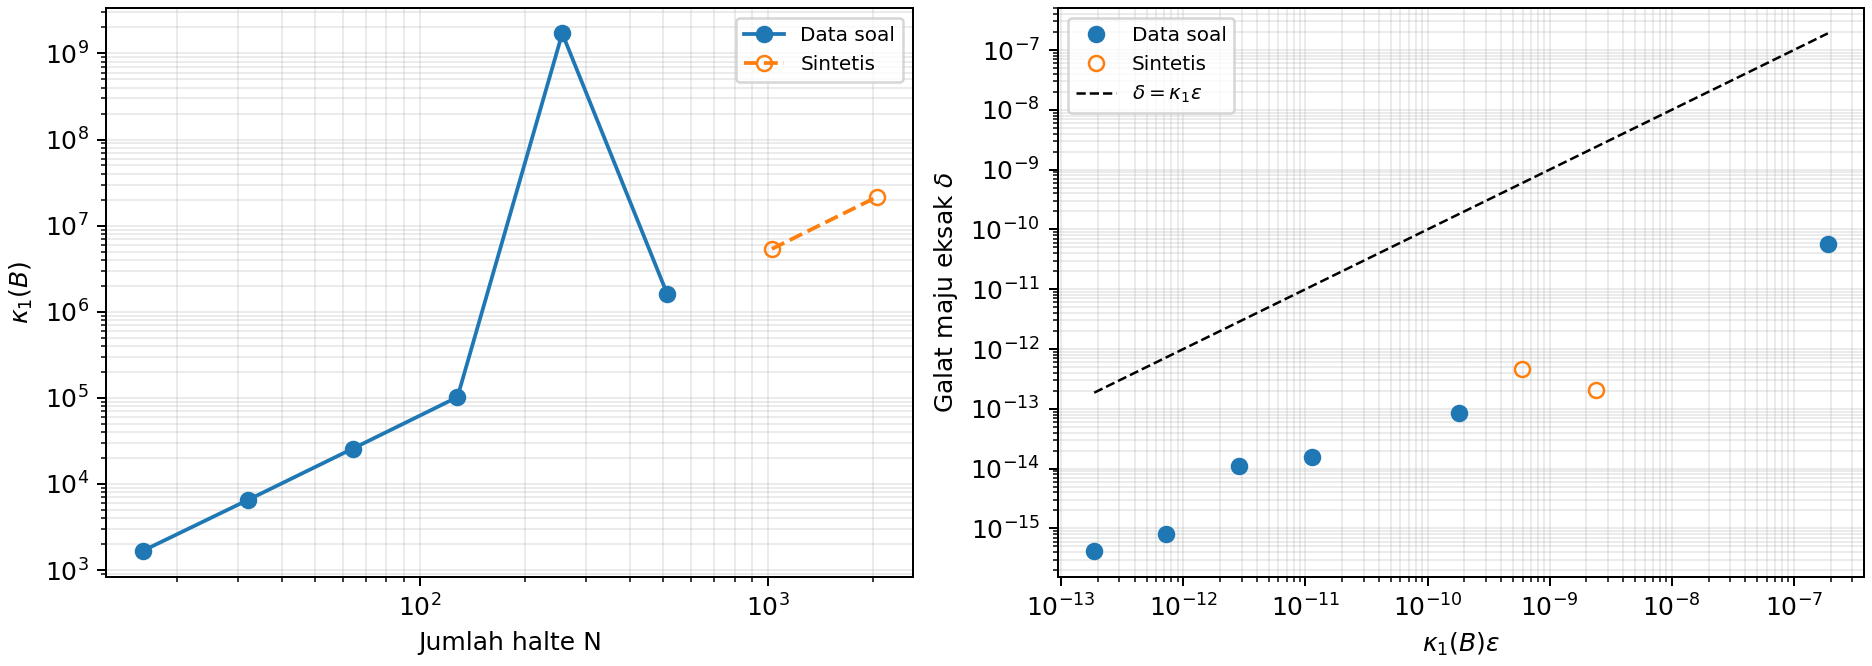
\includegraphics[width=.88\textwidth]{../soal1/hasil/kondisi_vs_N.png}
\caption{Bilangan kondisi terhadap $N$ dan galat maju terhadap batas kondisi.}\label{fig:kondisi-ringkas}
\end{figure}
\begin{figure}[H]\centering
\includegraphics[width=.88\textwidth]{../soal1/hasil/pi_vs_halte.png}
\caption{Profil distribusi stasioner terhadap nomor halte pada enam ukuran data.}\label{fig:pi-ringkas}
\end{figure}
Gambar~\ref{fig:kondisi-ringkas} menunjukkan lonjakan kondisi pada $N=256$, sedangkan Gambar~\ref{fig:pi-ringkas} memperlihatkan kenaikan $\pi_i$ ke arah ujung koridor. Halte terakhir memiliki proporsi terbesar pada keenam ukuran; pada $N=512$, $\pi_{512}\approx0.00301659$, sedangkan $\pi_1\approx0.00122645$. Massa menumpuk di ujung karena perpindahan maju tidak diimbangi oleh halte setelah $N$. Ini menunjukkan kebutuhan armada dan petugas relatif lebih tinggi di bagian akhir koridor; interpretasi tetap terbatas pada model transisi yang diberikan.

\section{Kesimpulan dan Rekomendasi}
Kedua solver akurat pada enam matriks uji. Solver pita adalah pilihan utama untuk jumlah halte besar karena memori dan operasi tumbuh linear pada lebar pita tetap, sedangkan LU dense tumbuh kuadratik dalam ruang dan kubik dalam waktu. Pemeriksaan $\kappa_1(B)$ tetap diperlukan: rantai hampir terpisah pada $N=256$ menunjukkan bahwa residual sangat kecil bisa menyertai sensitivitas solusi yang besar. Untuk data yang lebih buruk kondisinya, perbaikan iteratif atau algoritma GTH dapat dipertimbangkan~\cite{gth,higham}. Rekomendasi tersebut berdasarkan kompleksitas, waktu, memori, dan galat yang terukur; kedua teknik tambahan belum diuji di sini.
